\PassOptionsToPackage{unicode=true}{hyperref} % options for packages loaded elsewhere
\PassOptionsToPackage{hyphens}{url}
%
\documentclass[]{book}
\usepackage{lmodern}
\usepackage{amssymb,amsmath}
\usepackage{ifxetex,ifluatex}
\usepackage{fixltx2e} % provides \textsubscript
\ifnum 0\ifxetex 1\fi\ifluatex 1\fi=0 % if pdftex
  \usepackage[T1]{fontenc}
  \usepackage[utf8]{inputenc}
  \usepackage{textcomp} % provides euro and other symbols
\else % if luatex or xelatex
  \usepackage{unicode-math}
  \defaultfontfeatures{Ligatures=TeX,Scale=MatchLowercase}
\fi
% use upquote if available, for straight quotes in verbatim environments
\IfFileExists{upquote.sty}{\usepackage{upquote}}{}
% use microtype if available
\IfFileExists{microtype.sty}{%
\usepackage[]{microtype}
\UseMicrotypeSet[protrusion]{basicmath} % disable protrusion for tt fonts
}{}
\IfFileExists{parskip.sty}{%
\usepackage{parskip}
}{% else
\setlength{\parindent}{0pt}
\setlength{\parskip}{6pt plus 2pt minus 1pt}
}
\usepackage{hyperref}
\hypersetup{
            pdftitle={Tools for Analyzing Data},
            pdfauthor={Nicole Sorhagen, Ph.D.},
            pdfborder={0 0 0},
            breaklinks=true}
\urlstyle{same}  % don't use monospace font for urls
\usepackage{color}
\usepackage{fancyvrb}
\newcommand{\VerbBar}{|}
\newcommand{\VERB}{\Verb[commandchars=\\\{\}]}
\DefineVerbatimEnvironment{Highlighting}{Verbatim}{commandchars=\\\{\}}
% Add ',fontsize=\small' for more characters per line
\usepackage{framed}
\definecolor{shadecolor}{RGB}{248,248,248}
\newenvironment{Shaded}{\begin{snugshade}}{\end{snugshade}}
\newcommand{\AlertTok}[1]{\textcolor[rgb]{0.94,0.16,0.16}{#1}}
\newcommand{\AnnotationTok}[1]{\textcolor[rgb]{0.56,0.35,0.01}{\textbf{\textit{#1}}}}
\newcommand{\AttributeTok}[1]{\textcolor[rgb]{0.77,0.63,0.00}{#1}}
\newcommand{\BaseNTok}[1]{\textcolor[rgb]{0.00,0.00,0.81}{#1}}
\newcommand{\BuiltInTok}[1]{#1}
\newcommand{\CharTok}[1]{\textcolor[rgb]{0.31,0.60,0.02}{#1}}
\newcommand{\CommentTok}[1]{\textcolor[rgb]{0.56,0.35,0.01}{\textit{#1}}}
\newcommand{\CommentVarTok}[1]{\textcolor[rgb]{0.56,0.35,0.01}{\textbf{\textit{#1}}}}
\newcommand{\ConstantTok}[1]{\textcolor[rgb]{0.00,0.00,0.00}{#1}}
\newcommand{\ControlFlowTok}[1]{\textcolor[rgb]{0.13,0.29,0.53}{\textbf{#1}}}
\newcommand{\DataTypeTok}[1]{\textcolor[rgb]{0.13,0.29,0.53}{#1}}
\newcommand{\DecValTok}[1]{\textcolor[rgb]{0.00,0.00,0.81}{#1}}
\newcommand{\DocumentationTok}[1]{\textcolor[rgb]{0.56,0.35,0.01}{\textbf{\textit{#1}}}}
\newcommand{\ErrorTok}[1]{\textcolor[rgb]{0.64,0.00,0.00}{\textbf{#1}}}
\newcommand{\ExtensionTok}[1]{#1}
\newcommand{\FloatTok}[1]{\textcolor[rgb]{0.00,0.00,0.81}{#1}}
\newcommand{\FunctionTok}[1]{\textcolor[rgb]{0.00,0.00,0.00}{#1}}
\newcommand{\ImportTok}[1]{#1}
\newcommand{\InformationTok}[1]{\textcolor[rgb]{0.56,0.35,0.01}{\textbf{\textit{#1}}}}
\newcommand{\KeywordTok}[1]{\textcolor[rgb]{0.13,0.29,0.53}{\textbf{#1}}}
\newcommand{\NormalTok}[1]{#1}
\newcommand{\OperatorTok}[1]{\textcolor[rgb]{0.81,0.36,0.00}{\textbf{#1}}}
\newcommand{\OtherTok}[1]{\textcolor[rgb]{0.56,0.35,0.01}{#1}}
\newcommand{\PreprocessorTok}[1]{\textcolor[rgb]{0.56,0.35,0.01}{\textit{#1}}}
\newcommand{\RegionMarkerTok}[1]{#1}
\newcommand{\SpecialCharTok}[1]{\textcolor[rgb]{0.00,0.00,0.00}{#1}}
\newcommand{\SpecialStringTok}[1]{\textcolor[rgb]{0.31,0.60,0.02}{#1}}
\newcommand{\StringTok}[1]{\textcolor[rgb]{0.31,0.60,0.02}{#1}}
\newcommand{\VariableTok}[1]{\textcolor[rgb]{0.00,0.00,0.00}{#1}}
\newcommand{\VerbatimStringTok}[1]{\textcolor[rgb]{0.31,0.60,0.02}{#1}}
\newcommand{\WarningTok}[1]{\textcolor[rgb]{0.56,0.35,0.01}{\textbf{\textit{#1}}}}
\usepackage{longtable,booktabs}
% Fix footnotes in tables (requires footnote package)
\IfFileExists{footnote.sty}{\usepackage{footnote}\makesavenoteenv{longtable}}{}
\usepackage{graphicx,grffile}
\makeatletter
\def\maxwidth{\ifdim\Gin@nat@width>\linewidth\linewidth\else\Gin@nat@width\fi}
\def\maxheight{\ifdim\Gin@nat@height>\textheight\textheight\else\Gin@nat@height\fi}
\makeatother
% Scale images if necessary, so that they will not overflow the page
% margins by default, and it is still possible to overwrite the defaults
% using explicit options in \includegraphics[width, height, ...]{}
\setkeys{Gin}{width=\maxwidth,height=\maxheight,keepaspectratio}
\setlength{\emergencystretch}{3em}  % prevent overfull lines
\providecommand{\tightlist}{%
  \setlength{\itemsep}{0pt}\setlength{\parskip}{0pt}}
\setcounter{secnumdepth}{5}
% Redefines (sub)paragraphs to behave more like sections
\ifx\paragraph\undefined\else
\let\oldparagraph\paragraph
\renewcommand{\paragraph}[1]{\oldparagraph{#1}\mbox{}}
\fi
\ifx\subparagraph\undefined\else
\let\oldsubparagraph\subparagraph
\renewcommand{\subparagraph}[1]{\oldsubparagraph{#1}\mbox{}}
\fi

% set default figure placement to htbp
\makeatletter
\def\fps@figure{htbp}
\makeatother

\usepackage{booktabs}
\usepackage{amsthm}
\makeatletter
\def\thm@space@setup{%
  \thm@preskip=8pt plus 2pt minus 4pt
  \thm@postskip=\thm@preskip
}
\makeatother
\usepackage[]{natbib}
\bibliographystyle{apalike}

\title{Tools for Analyzing Data}
\author{Nicole Sorhagen, Ph.D.}
\date{2020-05-18}

\begin{document}
\maketitle

{
\setcounter{tocdepth}{1}
\tableofcontents
}
\hypertarget{about-gitbooks}{%
\chapter{About GitBooks}\label{about-gitbooks}}

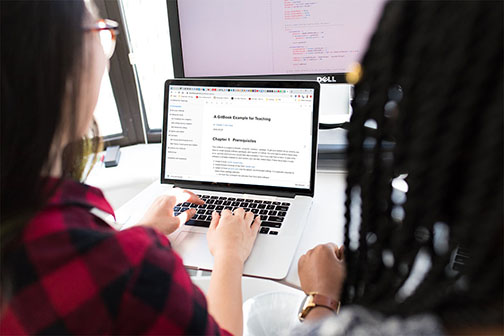
\includegraphics{./img/using_gitbook.jpeg}

A \emph{GitBook} is a useful tool for creating (open?) educational resources. It is an online ``book'' format, that can be hosted directly from a GitHub repository. You are currently reading a GitBook designed to help you get started creating your own educational GitBooks for your courses (how meta!). It does this in two ways: By explaining how to create GitBooks, and by serving as a template that you can copy and edit, instead of having to start from scratch. This template GitBook has all the settings that I consider to be useful for educational GitBooks, but you can always customize it.

I will focus specifically on GitBooks that are made in \href{https://rstudio.com}{Rstudio}, using the \href{https://rstudio.com/wp-content/uploads/2016/03/rmarkdown-cheatsheet-2.0.pdf}{\texttt{rmarkdown} markup language}, rendered using the \href{https://bookdown.org/yihui/bookdown/get-started.html}{\texttt{bookdown} package}, and hosted on \href{https://github.com/}{GitHub}. If you want to get started, skip ahead to Chapter \ref{prerequisites}; if you need more convincing, keep reading below.

\hypertarget{why-use-a-gitbook-for-teaching}{%
\section{Why use a GitBook for teaching?}\label{why-use-a-gitbook-for-teaching}}

\textbf{To spead the workload}

My challenge was that I had to translate all tutorial instructions from proprietary software to R, and there was not enough time to complete this task before the course commenced. By making the tutorial instructions available in \href{https://cjvanlissa.github.io/TCSM/}{this GitBook}, I was able to continue translating tutorial instructions \emph{while the semester was ongoing}, and push updates to GitHub in time for each session, which were immediately available to all students. The parallel with the current situation is that some courses are now forced to start teaching in an online format, without having enough time to completely prepare. By using a GitBook, you can spread out the workload of preparing your materials across the semester. \href{https://cjvanlissa.github.io/TCSM/}{This is the finished GitBook}

\textbf{To contribute or use existing Open Educational Resources}

Another key advantage of using a GitBook is, that you can easily make your course materials available for others to use under an open access license, or perhaps you can use an existing GitBook from the internet and adapt it for your own uses. GitBooks can be easily duplicated and adapted, just like any other project hosted on GitHub. Contributing Open Educational Materials can help reduce the workload on teachers around the world, and can improve the quality of the materials used thanks to online collaborating and feedback.

\textbf{To benefit from formatting advantages}

GitBooks also have two formatting advantages over classic PDF or Word files. First, they are Rmarkdown files, and can thus include blocks of R (\href{https://rstudio.github.io/reticulate/articles/r_markdown.html}{or Python}) code that can be evaluated, and whose results are rendered to the file. Second, they are interactive web pages, and as such, can have dynamic features (such as answers to assignments that can be hidden, or boxes where students can fill out an answer to be checked). Additionally, other web pages or interactive apps can be embedded within the page. So whereas a traditional document is static, GitBooks can be interactive.

\textbf{How do GitBooks work?}

GitBooks consist of an Rstudio project, with several Rmarkdown files containing the chapters of the book. Inside Rstudio, users can press a ``Build Book'' button, which renders all of these chapters to a nicely formatted HTML book (and a PDF file for users to download). Users can push the finished book to a GitHub repository, and indicate on GitHub that the book should be hosted on GitHub pages. Voilà!

\textbf{Getting started}

If you are convinced that this tool might benefit your teaching, your first point of action is to prepare your system for creating GitBooks (Chapter \ref{prerequisites}). After that, you can get a copy of this GitBook as a template (Chapter \ref{getgitbook}). Then, you can start tweaking it for your own course!

\hypertarget{set-up-project-on-rstudio-cloud}{%
\chapter{Set up project on Rstudio Cloud}\label{set-up-project-on-rstudio-cloud}}

First expand the R studio cloud options by clicking on the 3 lines in the top left corner.

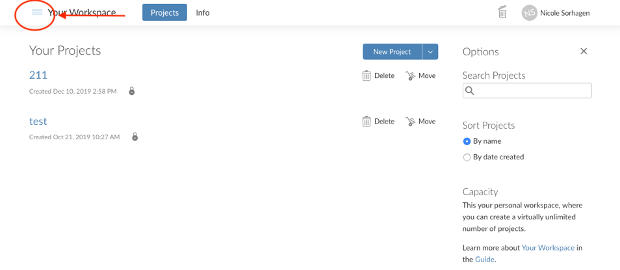
\includegraphics{img/Picture1.png}

\hypertarget{introduction-to-r}{%
\chapter{Introduction to R}\label{introduction-to-r}}

packages

library(tidyverse)

\hypertarget{getgitbook}{%
\chapter{Get your GitBook}\label{getgitbook}}

Test.

To get your GitBook, you should follow these steps:

\begin{enumerate}
\def\labelenumi{\arabic{enumi}.}
\tightlist
\item
  Go to \url{https://github.com/cjvanlissa/gitbook-demo}
\item
  In the top right of the page, click \texttt{Fork}.\\
  This will copy my \texttt{gitbook-demo} repository to your GitHub account.\\
  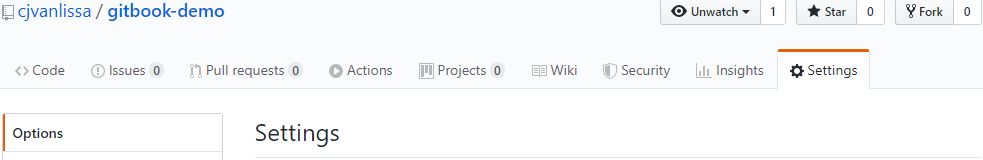
\includegraphics{./img/settings.png}
\item
  My repository is now copied to your account. It is a template repository, which means that you can create a \emph{new repository} based on this one.
\item
  Create a new repository for your own GitBook. Create one for a course you've been wanting to update. In the top-right corner of the GitHub website, click the + icon, and select ``New repository'':\\
  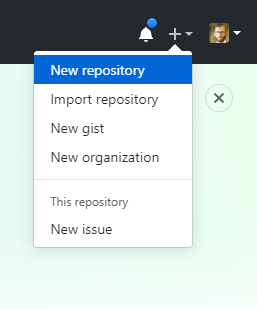
\includegraphics{./img/new_repo.png}
\item
  In the dialog, select the \texttt{gitbook-demo} as ``Repository template'', and give the repository an appropriate name for your course. Then, press \texttt{Create\ repository}:\\
  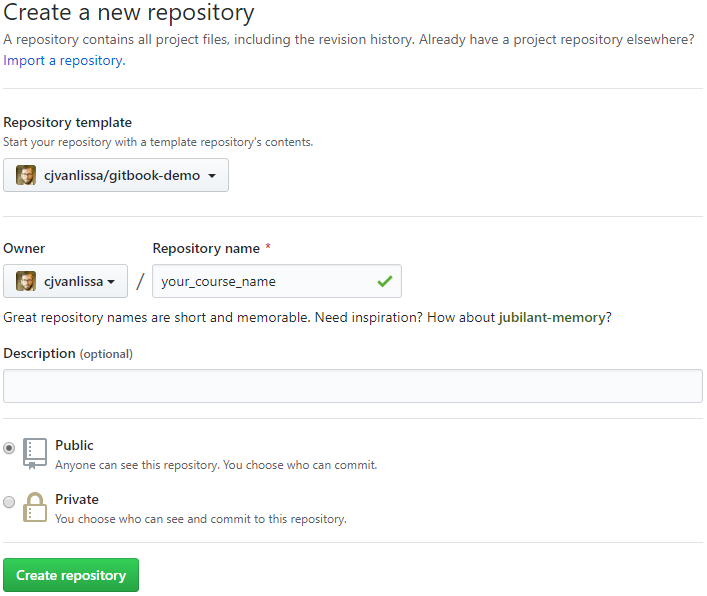
\includegraphics{./img/from_template.png}
\item
  Now, go back to Rstudio on your computer. In Rstudio, click \texttt{File\ \textgreater{}\ New\ Project}. A dialog will open. If you set up Rstudio with Git correctly, the dialog should have an option to create a new project from Version control. Click it:\\
  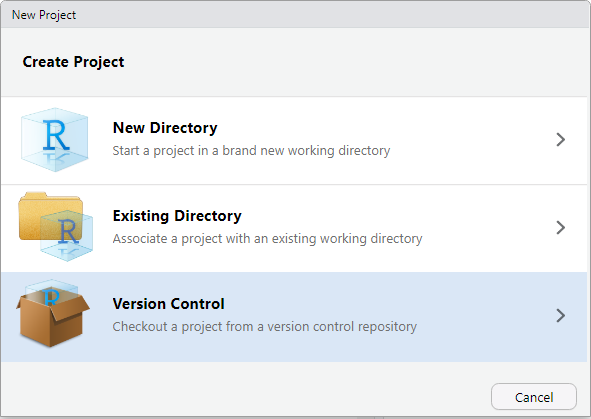
\includegraphics{./img/new_project.png}
\item
  In the next dialog window, you should copy the URL of the GitHub repository you created in \emph{Step 5}, like so:\\
  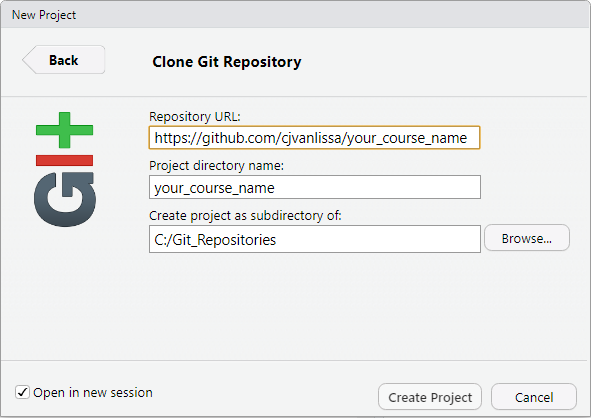
\includegraphics{./img/new_git_project.png}
\item
  Now, in Rstudio, you can open files for editing and create new files (explained in the next Chapter). Open files by clicking them in the Files editor (usually in the bottom right of Rstudio):\\
  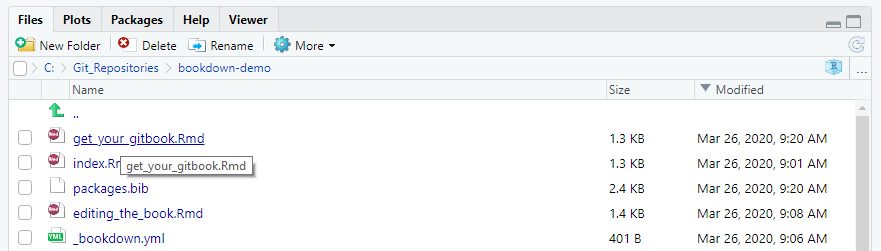
\includegraphics{./img/files_editor.png}
\item
  After you make a change, it will show up in the Git tab (usually in the top right of Rstudio). You must Commit the change locally, and then Push the change to GitHub to update your repo. To Commit, select the file and click the Commit button. Write a short message to describe the changes you made, then click the Commit button again. Now, press Push to send your commits to GitHub.\\
  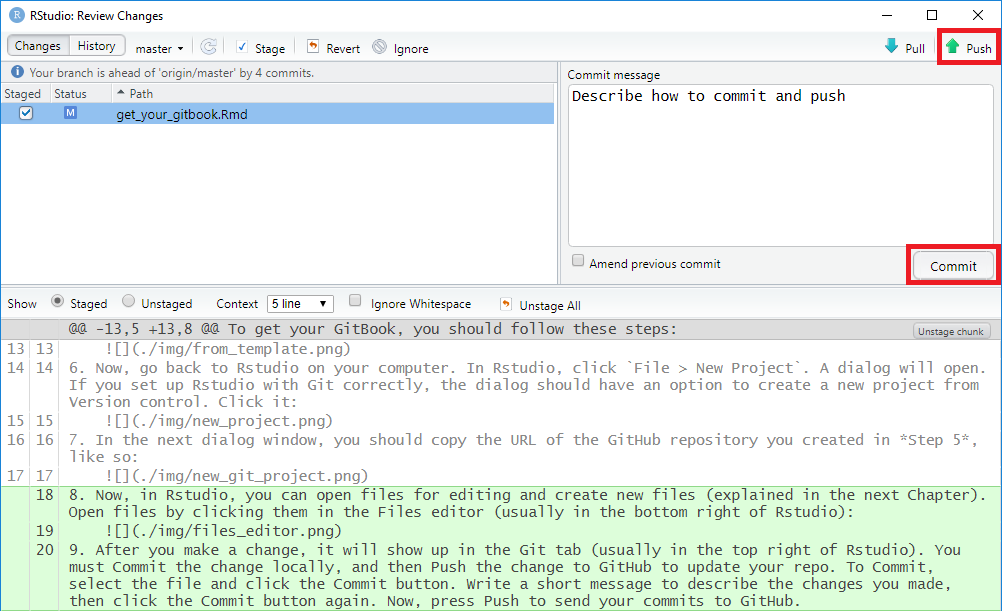
\includegraphics{./img/commit_push.png}
\item
  To render your book as a GitBook, you must ``Build'' it. In the top-right panel of Rstudio, you see a ``Build'' tab. In this tab, simply click the ``Build Book'' button to build your book. You should see a lot of rendering messages, until a window pops up with your brand new GitBook. If you get errors at this stage, you probably made a mistake in preparing your system (see the previous Chapter).\\
  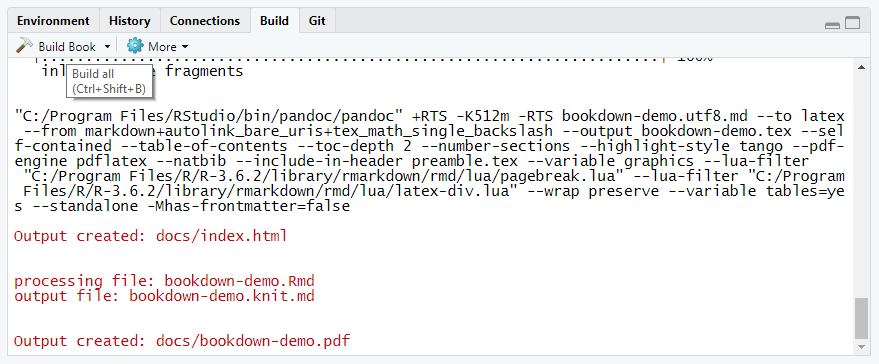
\includegraphics{./img/build_book.png}
\item
  Building the book generated a lot of new files in the \texttt{./docs} directory. This directory contains the website files for your GitBook. Open the Git tab again, verify that the \texttt{./docs} directory is listed, and Commit and Push all of these new files as described in \emph{Step 9}.
\item
  There is only one last remaining task: To publish your GitBook on GitHub pages. Once you do this, any change to the \texttt{./docs} folder that you push to GitHub will lead to an immediate update of your GitBook website. Go back to the GitHub page for your Repository. Click on the \texttt{Settings} tab on the top right of the page:\\
  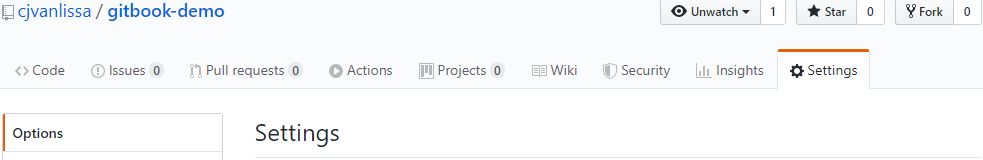
\includegraphics{./img/settings.png}
\item
  On the Settings page, scroll all the way down until you reach a section called \texttt{GitHub\ Pages}. There, under the ``Source'' heading, click the word \texttt{None}, and select \texttt{master\ branch\ /docs\ folder}. When you select it, the page will update, and if you scroll back down to the \texttt{GitHub\ Pages} section, you will see the URL where your GitBook is published. The first time, it will take a few minutes for your GitBook to come online. When you publish updates to the GitBook however (simply by following \emph{Step 11} again), the update will be near-instantaneous. The Pages section should now look like this (and that is hopefully the link where you found this book):\\
  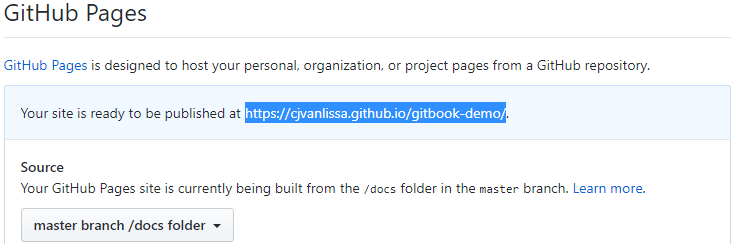
\includegraphics{./img/pages_published.png}
\end{enumerate}

\hypertarget{editing-the-book}{%
\chapter{Editing the book}\label{editing-the-book}}

The contents of the book are written in \textbf{RMarkdown}. You can use any formatting code that Pandoc's Markdown supports, e.g., a math equation \(a^2 + b^2 = c^2\). Moreover, you can include chunks of R-code, like this:

The results of these chunks can be rendered to the GitBook:

\begin{verbatim}
## [1] "This is an R-command!"
\end{verbatim}

To edit the book, you can change the text in the \texttt{.Rmd} files. Each Rmd file should contain \textbf{one and only one} chapter. A chapter is defined by the first-level heading \texttt{\#}, e.g., \texttt{\#\ Editing\ the\ book}.

Any sub-headings within the chapter are indicated with several \texttt{\#} signs, e.g., \texttt{\#\#} (level 2) and \texttt{\#\#\#} (level 3).

\hypertarget{creating-new-chapters}{%
\section{Creating new chapters}\label{creating-new-chapters}}

To create a new chapter, you must follow two steps: 1) Create the file, and 2) Include it in the list of chapters.

First, to create the file for a new chapter in Rstudio, click \texttt{File\ \textgreater{}\ New\ File\ \textgreater{}\ Text\ file}. At the top of the file, write your chapter heading, as explained above. Then, click \texttt{File\ \textgreater{}\ Save}. Save the file as \texttt{.Rmd}, without spaces in the file name, e.g.: \texttt{editing\_the\_book.Rmd}.

Second, to include it in the list of chapters, open the file \texttt{\_bookdown.yml} (click it in the Files explorer in the bottom right of Rstudio). This file has a list of \texttt{.Rmd} files to be included in the book. In this example, the list looks like this:

\begin{Shaded}
\begin{Highlighting}[]
\NormalTok{tmp <-}\StringTok{ }\KeywordTok{readLines}\NormalTok{(}\StringTok{"_bookdown.yml"}\NormalTok{)}
\KeywordTok{cat}\NormalTok{(tmp[}\KeywordTok{grep}\NormalTok{(}\StringTok{"^rmd_files"}\NormalTok{, tmp)}\OperatorTok{:}\KeywordTok{grep}\NormalTok{(}\StringTok{"references}\CharTok{\textbackslash{}\textbackslash{}}\StringTok{.Rmd"}\NormalTok{, tmp)], }\DataTypeTok{sep =} \StringTok{"}\CharTok{\textbackslash{}n}\StringTok{"}\NormalTok{)}
\end{Highlighting}
\end{Shaded}

rmd\_files: {[}``index.Rmd'',
``setuprstudiocloud.Rmd'',
``Introduction\_to\_R.Rmd'',
``get\_your\_gitbook.Rmd'',
``editing\_the\_book.Rmd'',
``figures\_tables.Rmd'',
``examples.Rmd'',
``open\_educational.Rmd'',
``use\_in\_course.Rmd'',
``licenses.Rmd'',
``references.Rmd''{]}

Insert the file name of your new chapter in the desired position in this list.

\hypertarget{linking-across-chapters}{%
\section{Linking across chapters}\label{linking-across-chapters}}

You can label chapter and section titles using \texttt{\{\#label\}} after them. The labels can be used as cross-references. For example, we can link to Chapter \ref{figtab}. If you do not manually label chapters, there will be automatic labels anyway, e.g., Chapter \ref{examples}.

\hypertarget{advanced-editing}{%
\section{Advanced editing}\label{advanced-editing}}

The convenient \href{https://rstudio.com/wp-content/uploads/2016/03/rmarkdown-cheatsheet-2.0.pdf}{Rmarkdown Cheat Sheet} by Rstudio covers most of the knowledge required for advanced Rmarkdown editing. You can print it out and stick it to your wall!

\hypertarget{figtab}{%
\chapter{Figures and tables}\label{figtab}}

Figures and tables with captions will be placed in \texttt{figure} and \texttt{table} environments, respectively.

\begin{Shaded}
\begin{Highlighting}[]
\KeywordTok{par}\NormalTok{(}\DataTypeTok{mar =} \KeywordTok{c}\NormalTok{(}\DecValTok{4}\NormalTok{, }\DecValTok{4}\NormalTok{, }\FloatTok{.1}\NormalTok{, }\FloatTok{.1}\NormalTok{))}
\KeywordTok{plot}\NormalTok{(pressure, }\DataTypeTok{type =} \StringTok{'b'}\NormalTok{, }\DataTypeTok{pch =} \DecValTok{19}\NormalTok{)}
\end{Highlighting}
\end{Shaded}

\begin{figure}

{\centering 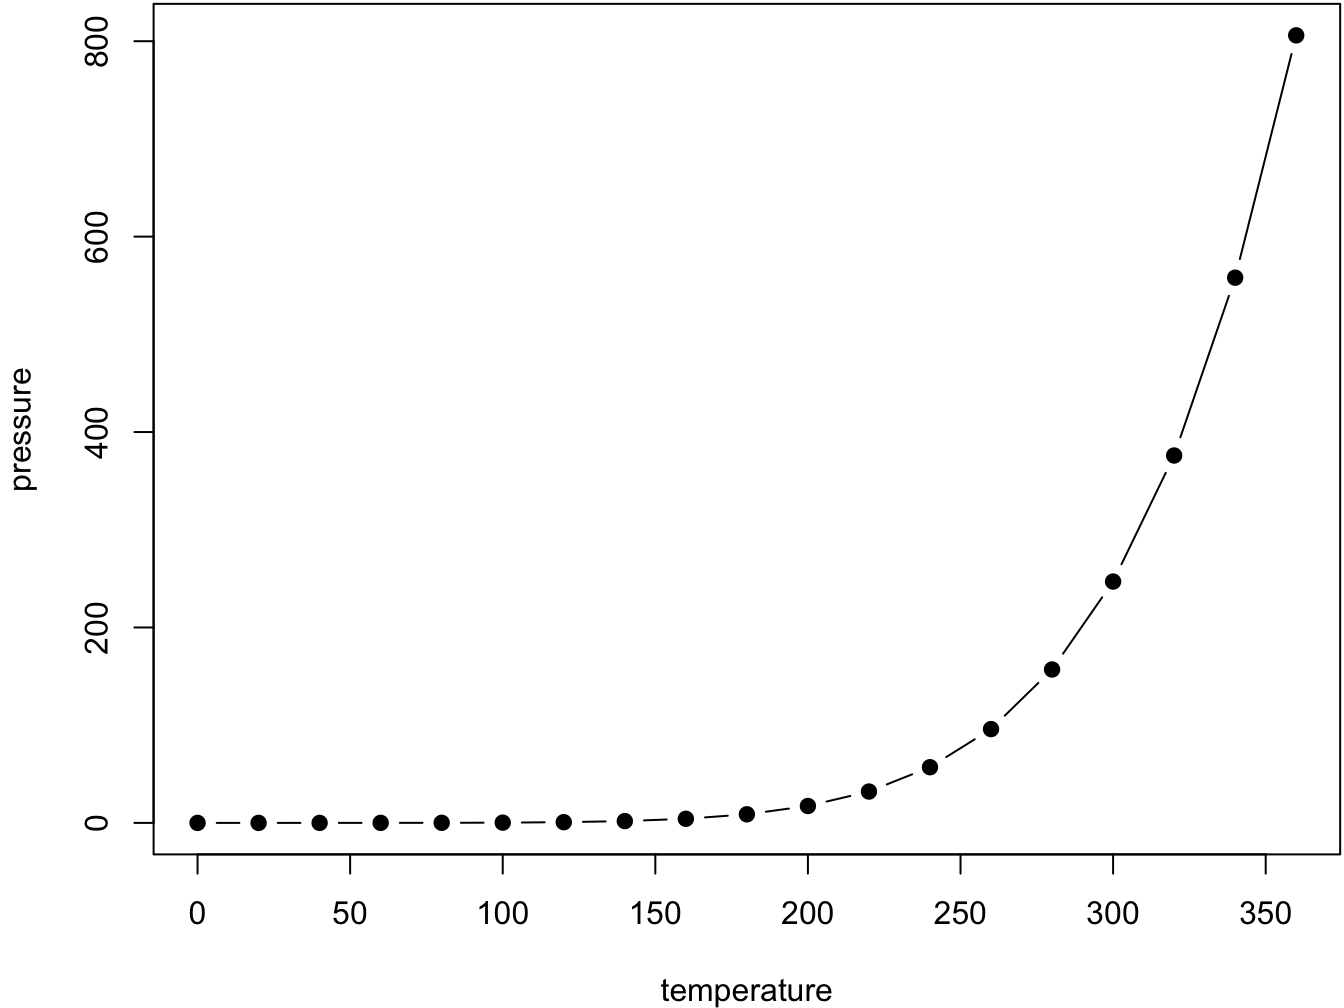
\includegraphics[width=0.8\linewidth]{Tools-for-Analyzing-Data_files/figure-latex/nice-fig-1} 

}

\caption{Here is a nice figure!}\label{fig:nice-fig}
\end{figure}

Reference a figure by its code chunk label with the \texttt{fig:} prefix, e.g., see Figure \ref{fig:nice-fig}. Similarly, you can reference tables generated from \texttt{knitr::kable()}, e.g., see Table \ref{tab:nice-tab}.

\begin{Shaded}
\begin{Highlighting}[]
\NormalTok{knitr}\OperatorTok{::}\KeywordTok{kable}\NormalTok{(}
  \KeywordTok{head}\NormalTok{(iris, }\DecValTok{20}\NormalTok{), }\DataTypeTok{caption =} \StringTok{'Here is a nice table!'}\NormalTok{,}
  \DataTypeTok{booktabs =} \OtherTok{TRUE}
\NormalTok{)}
\end{Highlighting}
\end{Shaded}

\begin{table}

\caption{\label{tab:nice-tab}Here is a nice table!}
\centering
\begin{tabular}[t]{rrrrl}
\toprule
Sepal.Length & Sepal.Width & Petal.Length & Petal.Width & Species\\
\midrule
5.1 & 3.5 & 1.4 & 0.2 & setosa\\
4.9 & 3.0 & 1.4 & 0.2 & setosa\\
4.7 & 3.2 & 1.3 & 0.2 & setosa\\
4.6 & 3.1 & 1.5 & 0.2 & setosa\\
5.0 & 3.6 & 1.4 & 0.2 & setosa\\
\addlinespace
5.4 & 3.9 & 1.7 & 0.4 & setosa\\
4.6 & 3.4 & 1.4 & 0.3 & setosa\\
5.0 & 3.4 & 1.5 & 0.2 & setosa\\
4.4 & 2.9 & 1.4 & 0.2 & setosa\\
4.9 & 3.1 & 1.5 & 0.1 & setosa\\
\addlinespace
5.4 & 3.7 & 1.5 & 0.2 & setosa\\
4.8 & 3.4 & 1.6 & 0.2 & setosa\\
4.8 & 3.0 & 1.4 & 0.1 & setosa\\
4.3 & 3.0 & 1.1 & 0.1 & setosa\\
5.8 & 4.0 & 1.2 & 0.2 & setosa\\
\addlinespace
5.7 & 4.4 & 1.5 & 0.4 & setosa\\
5.4 & 3.9 & 1.3 & 0.4 & setosa\\
5.1 & 3.5 & 1.4 & 0.3 & setosa\\
5.7 & 3.8 & 1.7 & 0.3 & setosa\\
5.1 & 3.8 & 1.5 & 0.3 & setosa\\
\bottomrule
\end{tabular}
\end{table}

You can write citations, too. For example, we are using the \textbf{bookdown} package \citep{R-bookdown} in this sample book, which was built on top of R Markdown and \textbf{knitr} \citep{xie2015}.

\hypertarget{examples}{%
\chapter{Examples}\label{examples}}

Here are some examples of other GitBooks for courses; if you want to have your GitBook added to the list, please send a \href{https://github.com/cjvanlissa/gitbook-demo/pulls}{Pull Request} (here's \href{https://help.github.com/en/github/collaborating-with-issues-and-pull-requests/creating-a-pull-request}{how to send a pull request}).

\hypertarget{statistics-with-r-h.-quene}{%
\section{Statistics with R (H. Quene)}\label{statistics-with-r-h.-quene}}

\url{https://hugoquene.github.io/emlar2020}

A GitBook for a tutorial on \emph{Statistics with R (Basics)}, held as part of the workshop on Experimental Methods in Language Acquisition Research (EMLAR, \url{https://emlar.wp.hum.uu.nl/}), Utrecht, on 17 April 2020. This compact introduction helps you with your first steps into R.

\hypertarget{theory-construction-and-statistical-modeling-c.-j.-van-lissa}{%
\section{Theory Construction and Statistical Modeling (C. J. van Lissa)}\label{theory-construction-and-statistical-modeling-c.-j.-van-lissa}}

\url{http://cjvanlissa.github.io/TCSM}

A GitBook for the course \emph{``Theory Construction and Statistical Modeling''}, with some interesting code, for example: Blocks of answers to the tutorial questions that can be collapsed and expanded.

\hypertarget{doing-meta-analysis-in-r-c.-j.-van-lissa}{%
\section{Doing Meta-Analysis in R (C. J. van Lissa)}\label{doing-meta-analysis-in-r-c.-j.-van-lissa}}

\url{http://cjvanlissa.github.io/Doing-Meta-Analysis-in-R}

A GitBook on doing meta-analysis in R, based on the book `Doing Meta-Analysis in R', by Mathias Harrer, Pim Cuijpers, \& David Ebert, and adapted to focus on the \href{https://cran.r-project.org/web/packages/metafor/index.html}{metafor} package, and exploring heterogeneity using \href{https://cran.r-project.org/web/packages/metaforest/index.html}{metaforest}. The original can be found here: \url{https://bookdown.org/MathiasHarrer/Doing_Meta_Analysis_in_R/}

\hypertarget{muxe9todos-quantitativos-em-psicologia-com-r-l.-anunciauxe7uxe3o}{%
\section{Métodos quantitativos em Psicologia com R (L. Anunciação)}\label{muxe9todos-quantitativos-em-psicologia-com-r-l.-anunciauxe7uxe3o}}

\url{https://anovabr.github.io/mqt/}

This book provides a short and to-the-point exposition on the essentials of statistics, and was written for undergraduate students at the Pontifical Catholic University of Rio de Janeiro (PUC-Rio). To a lesser degree, the mathematical modeling of statistical questions will be addressed. This book might be relevant for Portuguese-speaking students who enroll for laboratory-based statistics and anyone who wants to learn R.

\hypertarget{open-educational-resources}{%
\chapter{Open Educational Resources}\label{open-educational-resources}}

UNESCO defines Open Educational Resources as \href{https://en.unesco.org/themes/building-knowledge-societies/oer}{\emph{teaching, learning and research materials in any medium -- digital or otherwise -- that reside in the public domain or have been released under an open license that permits no-cost access, use, adaptation and redistribution by others with no or limited restrictions.}}

Open Educational resources can help lighten the workload on individual teachers, who can collaborate with the development of high-quality open access resources, instead of having to develop their own proprietary materials from scratch. Moreover, Open Educational resources are inclusive, lowering the barrier to knowledge acquisition for learners around the world, and enabling lifelong learning for those outside academia.

Many universities support Open Educational Resources. Here are just a few (feel free to \href{https://help.github.com/en/github/collaborating-with-issues-and-pull-requests/creating-a-pull-request}{send a pull request} with other relevant resources).

\begin{itemize}
\tightlist
\item
  \href{https://www.oercommons.org/}{\textbf{OER Commons}}: A freely accessible online library of open educational resources.
\item
  \href{https://uu.figshare.com/}{\textbf{Utrecht University Figshare}}: Open learning objects from Utrecht University.
\item
  \href{https://ocw.jhsph.edu/}{\textbf{Johns Hopkins University OCW}}: Open public health courses and materials.
\item
  \href{https://pitt.libguides.com/openeducation/biglist}{\textbf{University of Pittsburgh OER}}: Big List of Open Educational Resources.
\item
  \href{https://www.merlot.org/merlot/}{\textbf{MERLOT}}: Online learning and support materials and content creation tools, led by an international community of educators, learners and researchers.
\end{itemize}

\hypertarget{compatibility-with-existing-systems}{%
\chapter{Compatibility with existing systems}\label{compatibility-with-existing-systems}}

Many universities offer digital platforms for learning. You might wish to embed your GitBook within these existing systems. Here are two ways in which you might do that. Currently, this section only discusses BlackBoard, but the same principles should apply to other platforms.

\hypertarget{add-a-hyperlink}{%
\section{Add a hyperlink}\label{add-a-hyperlink}}

You can add a link to your GitBook in the BlackBoard course menu by following \href{https://help.blackboard.com/Learn/Instructor/Course_Content/Create_Content/Create_Course_Materials/Link_to_Websites}{this tutorial}.

\hypertarget{embed-the-whole-book}{%
\section{Embed the whole book}\label{embed-the-whole-book}}

You can add a Blank Page to your BlackBoard course menu, and fill that page with a full-size ``iframe'' - a web page within the web page. \href{https://mycampus.maine.edu/web/uc-faculty-portal/education-technology/-/asset_publisher/vEKuFJYvDY5K/content/inserting-an-iframe-into-blackboard?inheritRedirect=false}{This tutorial} explains how to do it. It is possible that your university is blocking this feature, however.

\hypertarget{license-your-gitbook}{%
\chapter{License your GitBook}\label{license-your-gitbook}}

In the spirit of Open Science, it is good to think about making your course materials Open Source. That means that other people can use them. In principle, if you publish materials online without license information, you hold the copyright to those materials. If you want them to be Open Source, you must include a license. It is not always obvious what license to choose.

The Creative Commons licenses are typically suitable for course materials. This GitBook, for example, is licensed under CC-BY 4.0. That means you can use and remix it as you like, but you must credit the original source.

If your project is more focused on software or source code, consider using the \href{https://www.gnu.org/licenses/gpl-3.0.en.html}{GNU GPL v3 license} instead.

You can find \href{https://creativecommons.org/share-your-work/licensing-examples}{more information about the Creative Commons Licenses here}. Specific licenses that might be useful are:

\begin{itemize}
\tightlist
\item
  \href{https://creativecommons.org/share-your-work/public-domain/cc0/}{CC0 (``No Rights Reserved'')}, everybody can do what they want with your work.
\item
  \href{https://creativecommons.org/licenses/by/4.0/}{CC-BY 4.0 (``Attribution'')}, everybody can do what they want with your work, but they must credit you. Note that this license may not be suitable for software or source code!
\end{itemize}

For compatibility between CC and GNU licenses, see \href{https://creativecommons.org/faq/\#Can_I_apply_a_Creative_Commons_license_to_software.3F}{this FAQ}.

\bibliography{book.bib,packages.bib}

\end{document}
